%!TEX root = ../main.tex
\label{section:moving_regions}

Real world examples of moving regions are everywhere. The movement of a car can be represented by a moving rectangle, forest fires, pollution areas and glacier extents can be represented by regions whose boundaries change over time, etc. Difficulties arise when we want to store and query these moving regions efficiently using moving object databases. Multiple different models have already been developed \cite{fmregion,polyhedra,model_structure_for_mod}, each one with positives and negatives. Most of these models make certain assumptions on the type of moving region or on the transformation that they undergo.

The literature makes a distinction between two major types of moving regions: deforming regions, analyzed and described by multiple authors \cite{polyhedra,model_structure_for_mod,moving_obj_foundation}, and fixed-shape regions, described in \cite{fmregion}. Another distinction that can be made is the difference between 2D and 3D regions. 

We will first discuss the difference between deforming and fixed-shape moving regions in the 2D case, and then briefly discuss 3D regions.

\section{Deforming Moving Regions}
\label{section:deforming_regions}

Deforming moving regions form a subset of the moving regions, and can be used in a large set of real-world application, such as the monitoring of forest fires, oil leaks in the ocean, flocks of birds, and many more. Depending on the application, these regions change in discrete steps, or continuously over time. 

When the regions change in discrete time steps, the major issue is the storage space, but there are no real other challenges, since the region is well-defined at every instant (using stepwise interpolation), and the usual spatial functions can be easily generalized to moving regions.

An example of a use case where a deforming moving region changes in discrete time steps is a cadastre. This type of moving regions is briefly discussed in Section \ref{section:deforming}. \\

When the regions are changing in a continuous manner, however, this stepwise interpolation method cannot be used anymore and a new interpolation method has to be defined. Next to this interpolation method, a storage model that allows to efficiently compute these interpolations has to be described as well. Since the start and end region might look very different, an additional difficulty arises when we want to construct the moving region from a set of snapshots. Indeed, the start and end regions can have a different number of vertices, and even a different number of faces if the region splits or merges.

The most common model used to represent a deforming moving region uses a \textit{sliced representation} \cite{algos_for_mod,model_structure_for_mod} (in the time axis) of the moving region, which defines a transformation from a start to an end region. There exist also ways of creating this sliced representation starting from snapshots of the moving region \cite{repr_from_obs}.

\begin{figure}[h!]
    \centering
    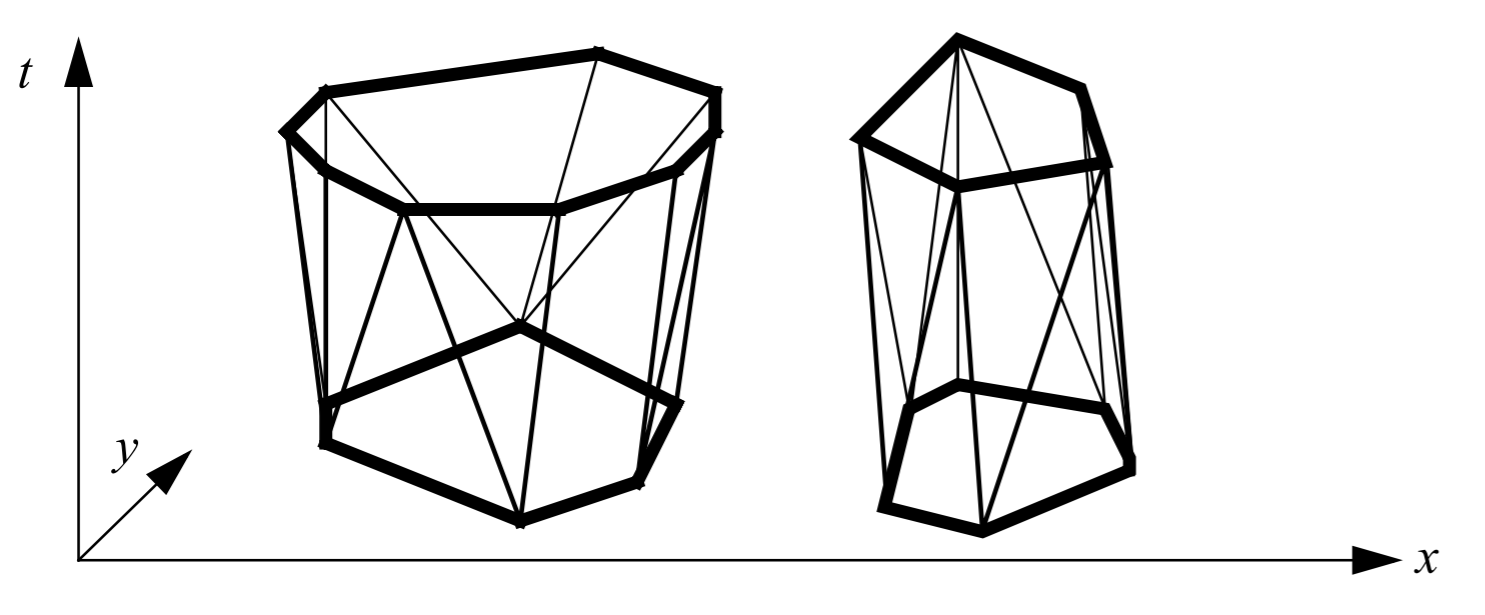
\includegraphics[width=0.75\textwidth]{images/sliced_moving_region.png}
    \caption[Sliced representation of moving regions]{Sliced representation of moving regions \cite{polyhedra}}
    \label{fig:sliced_repr_polygons}
\end{figure}

This slices representation of a moving regions makes use of \textit{moving segments}, which are pairs of \textit{moving points} that are co-planar in 3D space. This definition does not allow segments to rotate, but that can be avoided by representing a rotating segment using two moving segments.

\begin{figure}[h!]
    \centering
    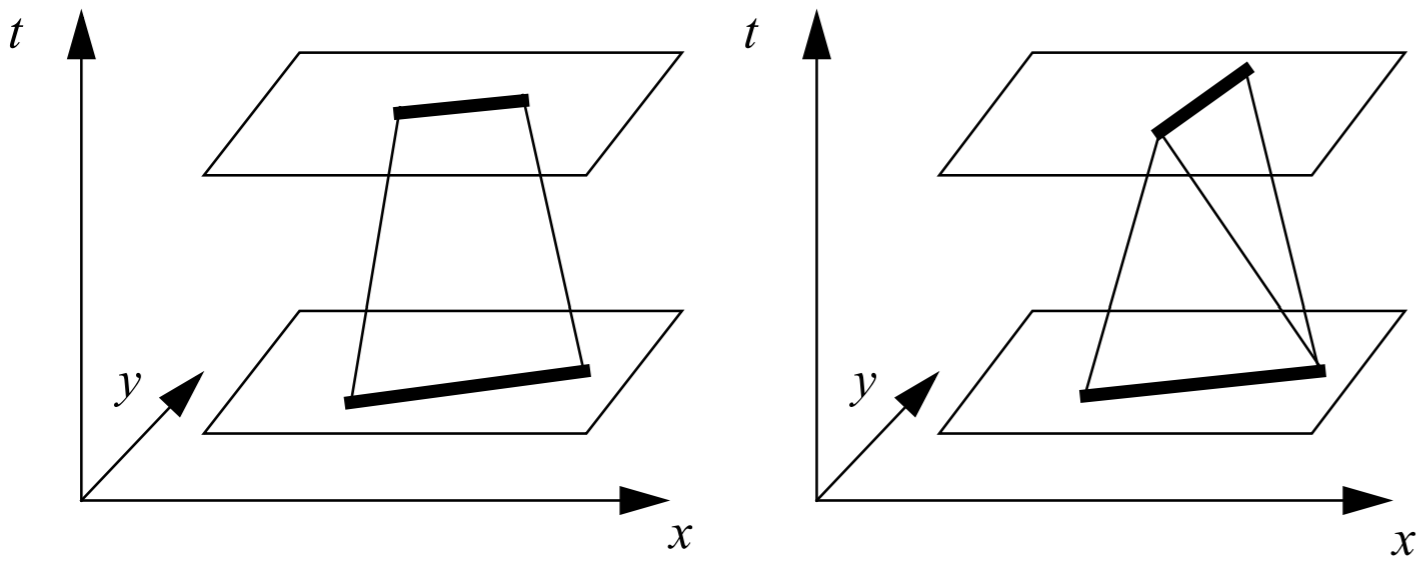
\includegraphics[width=0.75\textwidth]{images/sliced_moving_segments.png}
    \caption[Sliced representation of moving segments]{Sliced representation of moving segments, with rotating segments being represented using 2 distinct moving segments. \cite{polyhedra}}
    \label{fig:sliced_repr_segments}
\end{figure}


To describe the complete movement of a moving region or apply operations on these regions, many of these slices are needed, and this causes storage and efficiency issues. To solve this problem, a polyhedra-based model is described in \cite{polyhedra}, which uses the same moving segments as previously, but computes the operations more efficiently by using the temporal dimension as a third dimension, and using 3D geometry to compute the operations. As a result, less slices are created than in the previous implementations.

\section{Fixed-Shape Moving Regions}
\label{section:fixed_shape_regions}

Fixed-shape moving regions form another subset of all moving regions, and can be used to represent any moving rigid body, such a cars, boats, planes, etc. When the spatial extent of the object is negligible, and the orientation of no importance, the movement of such a body is usually represented by a moving point. When these conditions are not met, however, the movement of the region as a whole has to be analyzed.

The movement of fixed-shape regions can be described much easier than the movement of a deforming region, since the only possible transformations are translations and rotations. Theoretically, scaling could be taken into account too, but this case does not seem to have any real-world use case, so it is omitted.

Again, if the region moves in discrete time steps, the technical challenge only concerns the storage space, and here this can be efficiently resolved by storing the moving region as a polygon followed by a list of transformations. This technique is also used when handling continuous movement of regions, and is described below.

When we manage continuous moving regions, we again have to find a way to compute the interpolation efficiently. The previous model for deforming regions relies on moving segments, which are supposed to be non-rotating. This assumption is contradictory to the our idea of rotating (and translating) regions, and the larger the rotation of the region is, the worse the interpolation becomes. A good example of this is when a thin rectangle rotates 90 degrees without translating. The interpolation will considerably deform the region, which will at some point become a square, as can be seen in Figure \ref{fig:vertices_interpolation}.

\begin{figure}[h!]
    \centering
    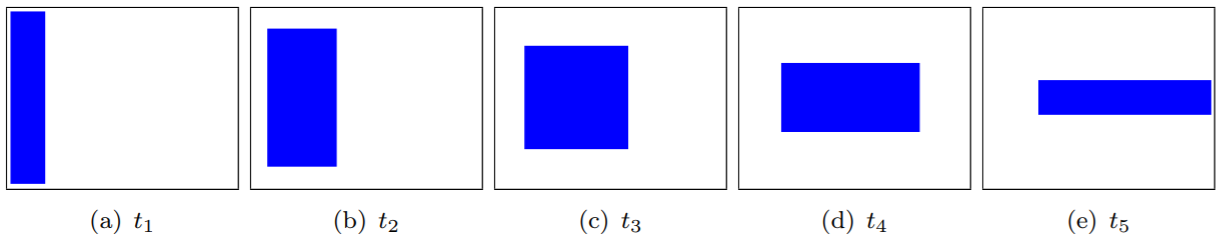
\includegraphics[width=0.75\textwidth]{images/vertices_interpolation.png}
    \caption[Linear interpolation of the vertices of a moving region]{Interpolation of a moving region using linear interpolation between the vertices. \cite{fmregion}}
    \label{fig:vertices_interpolation}
\end{figure}


The reason for this is that the interpolation method does not use the assumptions made on the possible transformations of the polygon. To solve this, a new model is proposed in \cite{fmregion}, which stores the region as a sequence of transformations, and makes use of these transformations to compute the correct interpolation. The resulting fixed-shape moving region is called \lstinline{fmregion} in this paper, and an example of a desired interpolation for this type of region is seen in Figure \ref{fig:fixed_shape_interpolation}.

\begin{figure}[h!]
    \centering
    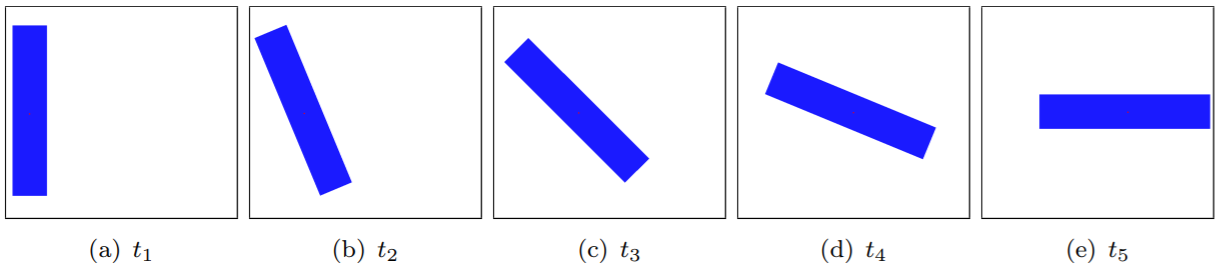
\includegraphics[width=0.75\textwidth]{images/fixed_shape_interpolation.png}
    \caption[Linear interpolation of a fixed-shape moving region]{Interpolation of a moving region using the fixed-shape assumptions. \cite{fmregion}}
    \label{fig:fixed_shape_interpolation}
\end{figure}


The model makes use of a \textit{transformationunit}, which specifies a rotation center $C$, an initial translation vector $v_0$ and rotation angle $\theta_0$, the vector $v$ and angle $\theta$ representing the transformation, as well as a time interval $[t_s; t_e]$, specifying the start and end instant of the transformation.

\[
    \textit{transformationunit } \mathcal{T}: (C, v_0, v, \theta_0, \theta, t_{s}, t_{e})
\]

An fmregion is thus defined by a single classical region $\mathcal{R}$ and a set of at least one transformation unit $\mathcal{T}$.

\[
    \textit{fmregion} : (\mathcal{R}, \mathcal{T}^{+})
\]

When computing the position of the region at a moment between the start and end instant of a transformation unit, the translation vector, and rotation angle are linearly interpolated, and then the transformation is applied to the initial region to retrieve the position of the region at the correct moment.

Note that the previous definition allows the region to rotate around an arbitrary rotation center for each transformation unit. This particularity allows the moving region to change rotation center between two transformation units, which is useful to describe a larger amount of trajectories than if the rotation center was fixed for all transformations. On the other hand, this also requires the user to input the rotation center for each transformation, since this cannot be uniquely computed by just seeing the start and end position of the region.

The same paper \cite{fmregion} also describes a few useful algorithms to process moving regions, such as a traversed area function, which computes the union of all places that the region went through during its movement.

\section{3D Moving Regions}
\label{section:3d_regions_intro}

The research articles presented in the two previous sections only focused on moving regions in two dimensions, but of course we might wonder if 3D moving regions could also be manipulated in a similar manner. Only 3D moving regions of fixed shape fixed-shape will be discussed here. To even just discuss about 3D deforming moving regions would require a much larger amount of research.

First of all, it is important to define what we call a 3D region. There is indeed a considerable difference between 3D polygons (polygons with points embedded in 3D space) and 3D polyhedra (3D volumetric objects). In the following, we will define a 3D region as a volumetric geometry, thus representable by a 3D polyhedron.

\begin{figure}[h!]
    \centering
    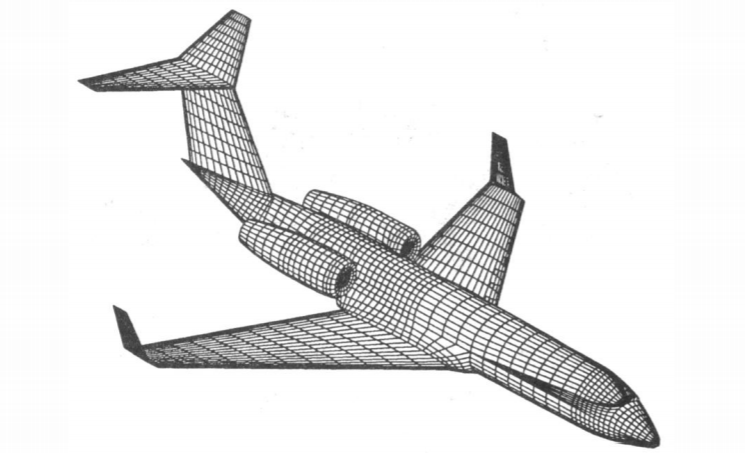
\includegraphics[width=0.75\textwidth]{images/plane_polyhedron.png}
    \caption[Representation of a plane using a 3D polyhedron]{Representation of a plane using a 3D polyhedron \cite{3d_polyhedron}}
    \label{fig:polyhedron}
\end{figure}


Support for 3D geometries is currently extremely restricted in database management systems \cite{3d_geom}. However, PostGIS does support two types of 3D geometries: \textit{Polyhedral Surfaces} and \textit{Triangulated Irregular Network Surfaces} [TIN], which are basically polyhedral surfaces where every polygon is a triangle. A few 3D functions are also implemented, such as \lstinline{ST_3DClosestPoint} or \lstinline{ST_3DDistance}.

First, let's look at the case where the regions move in discrete time steps. In this case, like previously, the problem of interpolating between two instants does not arise, and the difficulty is reduced to storing the large amount of data that might be present in an efficient manner. 

If we assume fixed-shape regions, we can again use the fact that the only possible transformations are translations and rotations. It is thus sufficient to store the region once as a 3D polyhedron, and then store only the difference in position and orientation for all other positions. This technique is similar to the one described in the previous section, except that the translation and rotation is done in 3D space instead of 2D.

Looking at continuously moving regions, we can apply the same storage idea, and retrieving the position of the region between two stored instants by computing a linear interpolation of the translation, just as was done in 3D, and computing a more advanced interpolation for the 3D rotation, based on \textit{quaternions}.

This interpolation method will be discussed in a later section (Section \ref{section:3d_regions}), but the important part is that it can be done. Storing 3D moving regions of fixed-shape is thus possible, and retrieving the region at any arbitrary instant is too. Implementation of functions that can manipulate and analyze these regions is another issue, and is left as future research.